\newcommand{\sol}{_{\odot}}
\newcommand{\Msol}{$M\sol { }$}


%\part*{Lezione 11/03/2021}
\chapter{Big Bang Nucleosynthesis}\label{cap-BBN}

\paragraph{Astronomical Observations}
Riportiamo adesso alcune informazioni generali su osservazioni astronomiche che ci serviranno per poterci poi concentrare sulla nucleosintesi primordiale e sulle reazioni all'interno delle stelle.



\begin{itemize}
    \item La Via Lattea\index{Via Lattea} è una galassia a spirale larga circa 30 kpc\footnote{Le misure sono riportate in \textit{parsec}\index{parsec}; ricordiamo che:
    $$1 \unit{pc} = 3\cdot 10^{16} \unit{m} = 3.3 \unit{ly}$$%
    } e spessa 1 kpc. \`E composta da $2\cdot 10^{11}$ stelle, polveri e gas. Il Sole è situato a circa 8.5 kpc dal centro galattico, che consiste in un buco nero supermassiccio\footnote{Se non fosse per il mezzo interstellare avrebbe una luminosità apparente pari a quella del Sole.} chiamato Sgr A$^*$\index{Sgr A$^*$}. La nostra Galassia insieme alla galassia di Andromeda\index{galassia di Andromeda} e una ventina di altre galassie nane forma il Gruppo Locale\index{Gruppo Locale}; questo è legato (gravitazionalmente) a sua volta ad altri gruppi con cui forma l'Ammasso della Vergine\index{Ammasso della Vergine} per un totale di circa $10^{10}$ galassie che occupano circa il $5\%$ dell'Universo.\\
    Le masse in gioco sono:
    $$M\sol\sim 2\cdot10^{30} \unit{kg}, \;\; \rho\sol \sim \rho_{\ce{H_2O}} \qquad M_{MW} > 2\cdot 10^{11} M\sol$$
    come abbiamo detto, non sono presenti solo stelle nella Via Lattea, ma anche mezzo e materia oscura. Per quanto riguarda il gas\index{gas@gas del mezzo interstellare}, questo ha una densità che varia da $10^9$ atomi/m$^3$ vicino al sistema solare fino a circa $10^5$ altrove e contiene principalmente H ed He con tracce di molecole.
    \item L'analisi spettrale\index{analisi spettrale} mi dà informazioni sulla temperatura e la composizione chimica.
    \item La luminosità\index{luminosità} è la densità di flusso di energia: $L = 4\pi R^2 \sigma\, T_{sup}^4$ dove $\sigma \equiv 5.7\cdot10^{-8}$ Wm$^{-2}$K$^{-4}$ è  la costante di Stefan-Boltzmann\index{costante di Stefan-Boltzmann@costante di Stefan-Boltzmann $\sigma$}; per cui:
    $$\Bigl ( \frac{L}{L\sol} \Bigr ) = \Bigl ( \frac{R}{R\sol}\Bigr )^2 \; \Bigl (\frac{T}{T\sol} \Bigr )^4$$
    Da questa relazione è possibile costruire un diagramma temperatura-luminosità detto diagramma Hertzsprung-Russell\index{diagramma Hertzsprung-Russell} in Figura \ref{0311_herz}. In questo grafico si osserva che le stelle in \textit{main sequence}\index{main sequence@\textit{main sequence}} si collocano quasi su una retta. Le rette grige corrispondono a linee lungo le quali si ha un raggio costante.
    \begin{figure}[h]
    \centering
    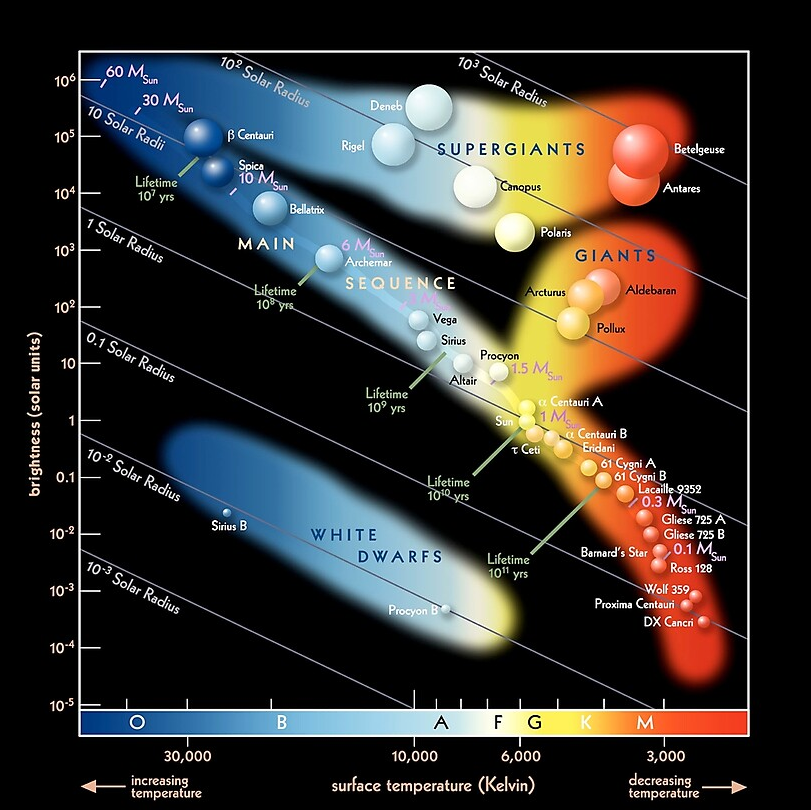
\includegraphics[scale=0.4]{Immagini/0311_herzprung1.png}
    \caption{Diagramma di Hertzsprung-Russell}
    \label{0311_herz}
    \end{figure}
    \item Nel 1930 Hubble si rende conto che le galassie sono uniformemente distribuite nel cielo\footnote{Da questo nascerà il Principio Cosmologico\index{Principio Cosmologico} per cui l'Universo viene assunto uniforme e isotropo (su \vir{grandi} scale).} e che si stanno allontanando. Tale deriva è osservabile dall'effetto Doppler\index{effetto Doppler} sulle righe spettrali di queste galassie, ovvero uno spostamento verso \vir{il rosso} (lunghezze d'onda maggiori); si definisce allora il parametro di \textit{redshift}\index{parametro di redshift@parametro di \textit{redshift} $z$}:
    $$z\equiv \frac{\lambda(v) - \lambda(0)}{\lambda(0)}\simeq \frac{v}{c}$$
    con $v\ll c$. Dalle osservazioni si evince che $z$ è proporzionale alla distanza $d$ dell'oggetto; la costante di proporzionalità tra la velocità di allontanamento e la distanza è detta costante di Hubble $H$\index{costante di Hubble@costante di Hubble $H$}. Sul valore di questa costante c'è tensione, riportiamo il valore ottenuto dalla misura sulle scale di distanza: $H= 72\unit{km}\,\mbox{s}^{-1}\mbox{Mpc}^{-1} \simeq 2.3\cdot 10^{-18}\unit{s}^{-1}$. Ipotizzando che il rate di espansione sia rimasto sempre lo stesso allora $H^{-1}$ dà una stima dell'età dell'universo $t\sim 12 \cdot 10^9\unit{y}$.
    \item Nasce così l'idea (riavvolgendo nel tempo l'espansione) di un punto di inizio da cui tutto è partito: il \textit{Big Bang}\index{Big Bang@\textit{Big Bang}}. Secondo questa teoria, materia e radiazione erano inizialmente accoppiate fino a un tempo di disaccoppiamento e di successiva ricombinazione tra i barioni. Da quel momento in poi la radiazione (su larga scala) non ha più interagito con la materia e infatti si osserva un fondo di radiazione cosmica detto \textit{Cosmic Microwave Background}\index{Cosmic Microwave Background@Cosmic Microwave Background CMB} (CMB), ancora oggi molto studiato. La teoria prevedeva\footnote{Questi valori dipendono fortemente dal modello.} una $\lambda\simeq 7.5\unit{cm}$ (da cui il nome \textit{microwave}), che per un corpo nero corrisponde a $T\simeq 2.7\unit{K}$, e fu osservato nel 1965 da Penzias e Wilson. 
    \item Per misurare $H_0$ (dove il pedice indica che la costante è misurata per il tempo attuale) si utilizzano principalmente 2 metodi: l'osservazione dell'espansione dell'Universo dagli spettri delle galassie lontane oppure delle disomogeneità nel CMB.
    Nel primo caso, è necessario selezionare galassie per cui la velocità di espansione è più rilevante rispetto alla velocità peculiare\index{velocità peculiare}\footnote{Si tratta della velocità di avvicinamento dovuta alle interazioni gravitazionali tra galassie ed è dell'ordine del 100 km/s.} e misurarne le distanze; a tal scopo si fa uso di candele campione\index{candela campione} (oggetti con poca astrofisica, ben identificabili) e dalla legge di Hubble\index{legge di Hubble} ottengo una stima indipendente dal modello cosmologico di $H_0$.\\ 
    Nel metodo della CMB, invece, si osservano le sovradensità dovute a fluttuazioni in densità dell'ordine di $10^{-2}$ nell'Universo primordiale che hanno portato a un gradiente di pressione, quindi a onde sonore; al momento della ricombinazione queste oscillazioni si sono congelate e ci aspettiamo quindi dei picchi in queste fluttuazioni detti appunto \textit{acoustic peaks}\index{acoustic peaks@\textit{acoustic peaks}}, visibili per alcuni $\Vec{k}$ tramite un'analisi spettrale, come mostrato in Figura \ref{0311_peak}. Questi picchi dipendono da alcuni parametri cosmologici tra cui $\Omega_b$ che è legata alla densità critica $\rho_c\equiv 3H_0^2/8\pi G$\index{densità critica@densità critica $\rho_c$}, per cui si ottiene una stima di $H_0$, ma che dipende fortemente dal modello. Come si vede in Figura \ref{0311_H0} vi è tensione e ancora oggi si sta cercando una risposta.
    \begin{figure}[h]
        \centering
        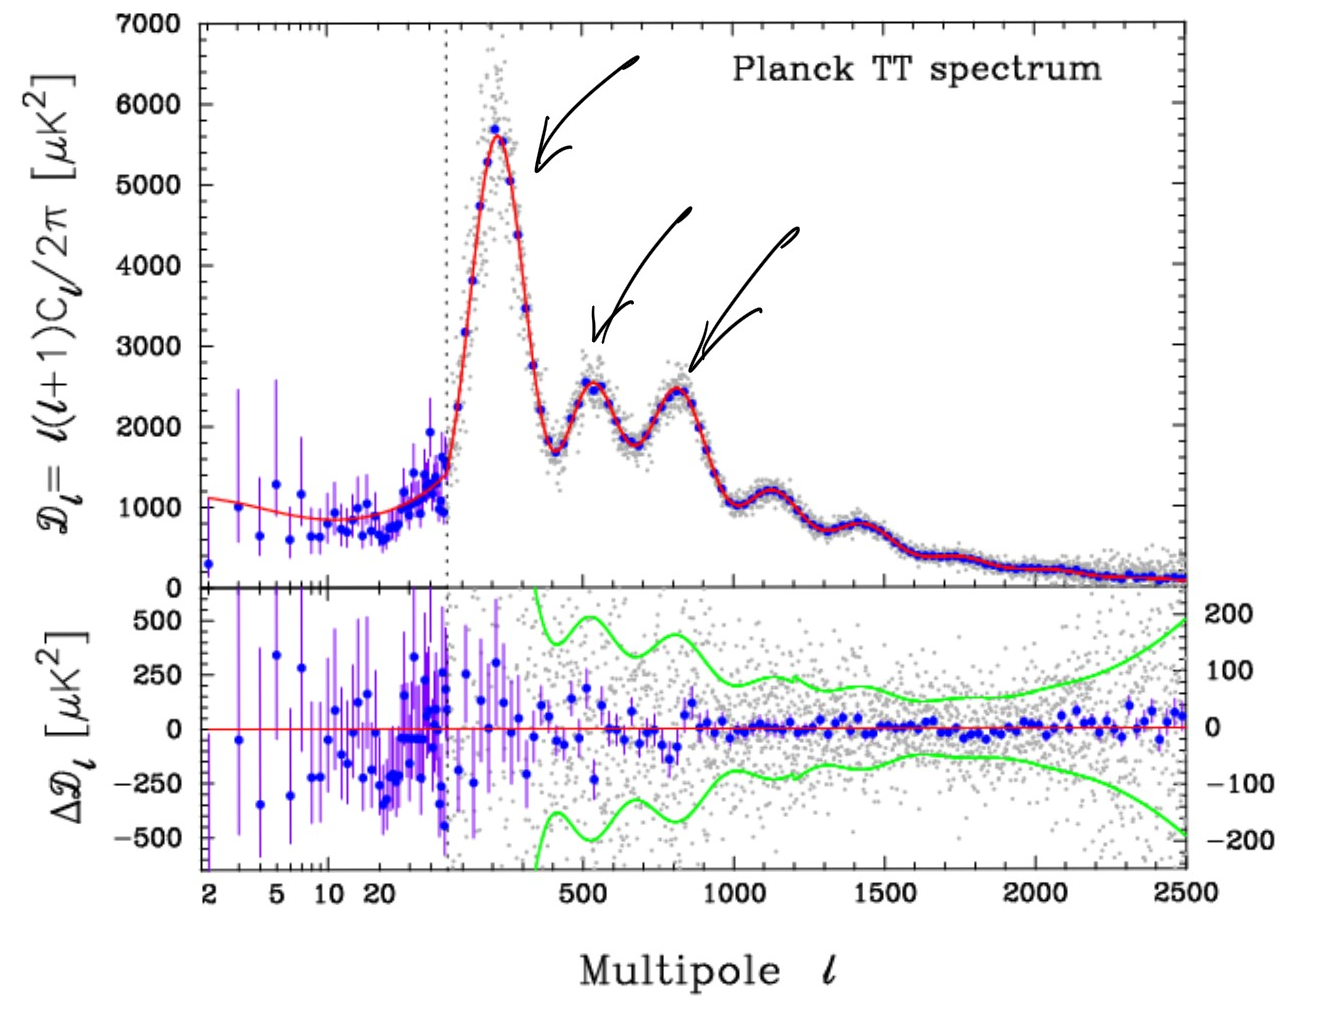
\includegraphics[scale=0.2]{Immagini/0311_peak.png}
        \caption{Analisi spettrale della sovradensità nel CMB. Si possono osservare i picchi di cui parlavamo.}
        \label{0311_peak}
    \end{figure}
    \begin{figure}[h]
        \centering
        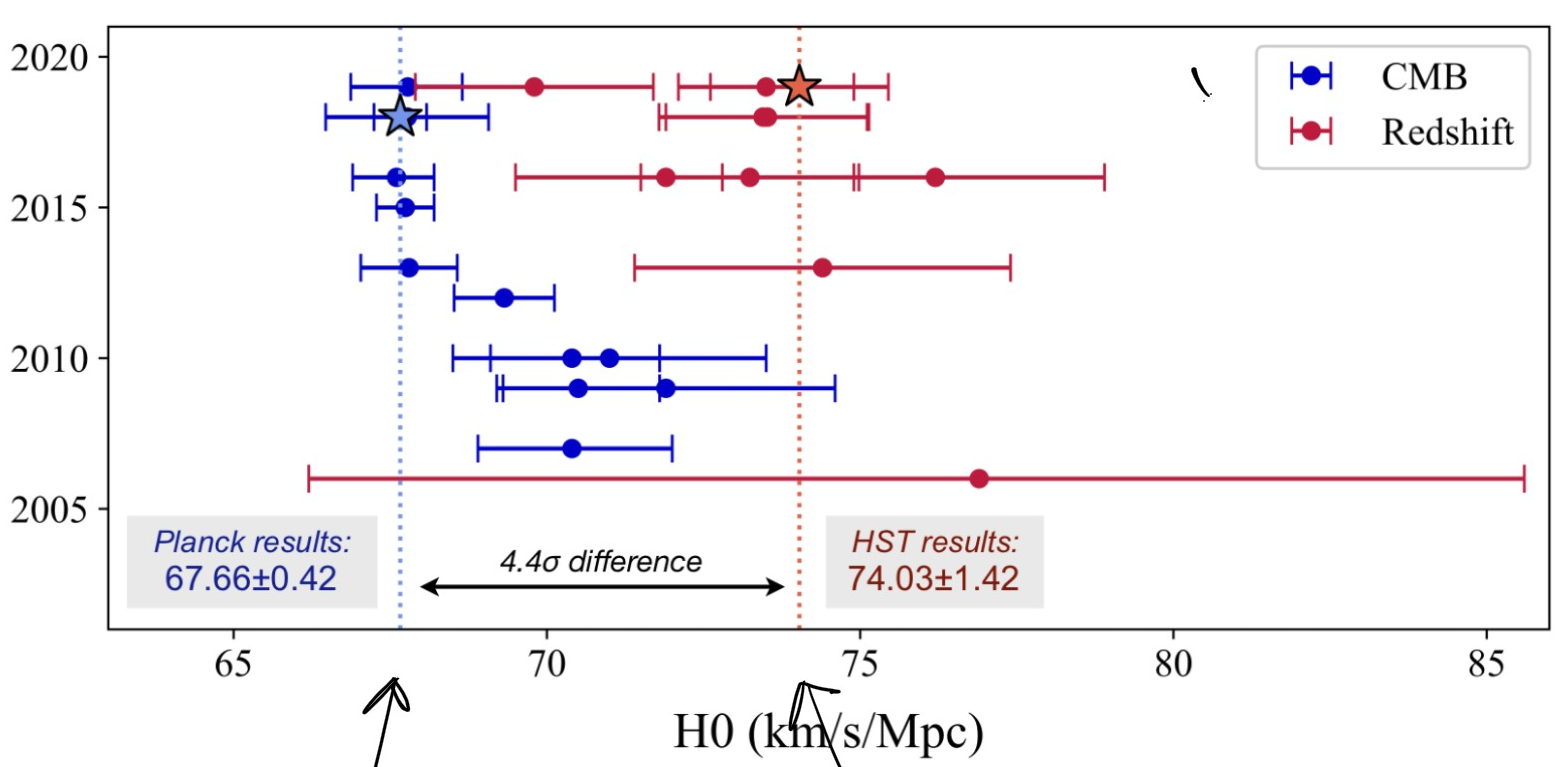
\includegraphics[scale=0.2]{Immagini/0311_peak2.png}
        \caption{Tensione per le misure di $H_0$. Si osserva che nel tempo i valori si sono allontanati.}
        \label{0311_H0}
    \end{figure}
\end{itemize}
\noindent Queste osservazioni ci hanno portati alla teoria del \textit{Big Bang}, necessaria per introdurre il prossimo fondamentale argomento, ovvero la trattazione dei meccanismi e delle tipologie delle reazioni nucleari che hanno caratterizzato l'Universo primordiale, detta \textit{\textbf{Big Bang Nucleosynthesis Theory}}\index{Big Bang Nucleosynthesis} (\textbf{BBN}).


\section{Introduzione alla teoria}
Il \textit{Big Bang model} comporta necessariamente la formulazione di una teoria sulla nucleosintesi primordiale. Questa fu trattata per la prima volta in un articolo del 1940 degli autori Gamow, Adler e Bethe\index{articolo Adler, Bethe, Gamow@articolo $alpha,\,\beta,\,\gamma$}\footnote{Un aneddoto diverte: Gamow (che è lo stesso Gamow del decadimento di Gamow-Teller\index{decadimento!Gamow-Teller}) insistette per avere la partecipazione anche di Bethe, per poter mettere nell'articolo i nomi \vir{Adler, Bethe, Gamow} che ricordavano $\alpha,\,\beta,\,\gamma$, nome con cui ormai viene ricordato l'articolo.}.

\paragraph{Il problema di $Y_P$} Prima di passare allo studio delle reazioni di interesse, mostriamo come alcuni risultati confermano la necessità di una nucleosintesi primordiale.\\
Se assumiamo che $M_{MW} \sim 10^{11}$ \Msol e $L_{MW}\sim 2\cdot \ord{10}\unit{L}\sol {}$ allora l'energia totale liberata in un tempo $H_0^{-1}$ sarà $E_{tot} \simeq L_{MW}/H_0\sim 2.4\cdot 10^{54}\unit{J}$; escludendo la nucleosintesi primordiale l'unica reazione possibile è $4p\to\ce{^4He}$, allora $E_{\ce{^4He}} = 28\unit{MeV}= 4.5 \cdot \ord{-12}\unit{J}$. Se tutta la massa stellare bruciasse allora si libererebbe un'energia pari a $E_{burn} \equiv E_{\ce{^4He}}\cdot M_{MW}/4m_p\sim 1.3\cdot \ord{56}\unit{J}$, da cui otteniamo $E_{tot}/E_{burn}\sim 2\%$ che corrisponde alla percentuale in massa di $\ce{^4He}$ \vir{primordiale} $Y_P$. Tuttavia, sperimentalmente si osserva che $Y_P\simeq 25\%$, dunque le reazioni nucleari nei core stellari non sono sufficienti per spiegare questa abbondanza ed è necessario introdurre un altro meccanismo (la nucleosintesi primordiale, appunto).

\paragraph{A grandi linee}\label{a.grandi.linee} Proviamo a correggere il risultato precedente con argomentazioni qualitative. Ovviamente per la nostra trattazione non siamo interessati al \textit{Big Bang}\index{Big Bang@\textit{Big Bang}}, ma fisseremo come origine dei tempi l'attimo prima che protoni e neutroni si formino: 
\begin{itemize}
    \item a $t=0\unit{s}$ abbiamo quindi una sfera molto densa e molto calda $T>\ord{13}\unit{K}$.  
    \item a $t\sim 0.01\unit{s}$ domina ancora la radiazione e non riescono a formarsi protoni e neutroni perché $T\sim\ord{13}$ quindi $E=kT\sim 1\unit{GeV}$, quindi anche se ci fossero $p$ e $n$ verrebbero fotodisintegrati.
    \item a $t\sim 0.1\unit{s}$ la temperatura scende a $T\sim 3\cdot\ord{10}\unit{K}$ per cui $E\simeq 3\unit{MeV}$ e si formano finalmente protoni e neutroni.\\ 
    A questo punto è fondamentale ricordare che la massa del neutrone è maggiore di quella del protone $\Delta m = 1.3\unit{MeV}$ per cui avremo al momento del \textit{Freeze-out}\index{Freeze-out@\textit{Freeze-out}}:
    $$\frac{N_n}{N_p}\propto \exp{\ppc{-\frac{\Delta m}{kT}}} \simeq 0.22 \simeq \frac{1}{5}$$
    per cui per 1000 protoni abbiamo 220 neutroni circa. Ancora non si può formare il deutone.
    \item a $t\sim 180\unit{s}$ la temperatura raggiunge $T\sim \ord{9}\unit{K}$ a cui corrisponde $E\sim 0.09\unit{MeV}$ e quindi si possono formare i nuclei. Tuttavia, è necessario ricordare che il neutrone decade con una legge del tipo $N_n(t) = N_n^0 \, \exp{(-t/\tau_n)}$ con $\tau_n \sim 886\unit{s}$; nell'esempio da noi fatto ($N_n^0= 220$) avremo $N_n \simeq 180$ e $N_p = N_p^0 + (N_n^0-N_n) = 1040$.
\end{itemize}
\noindent Allora possiamo ipotizzare che qualitativamente\footnote{In realtà esiste un \textit{full network} di relazioni.} avremo queste relazioni:
\begin{displaymath}
\begin{aligned}
n + p &\to d + \gamma \\
n + d &\to \ce{^3H} + \gamma \\
\ce{^3H} + p &\to \ce{^4He} + \gamma
\end{aligned}
\end{displaymath}
Ci chiediamo quanto valga $Y_P$:
\begin{displaymath}
\begin{aligned}
Y_P &= \frac{4 N_{\ce{He}}}{N_{p,\text{rimasto} + 4N_{\ce{He}} }} \;\leftarrow\: \text{Mass fraction}\\
&= \frac{4 \frac{N_n}{2}}{(N_p - N_n) + 4\frac{N_n}{2}} = \\
&\simeq 0.29
\end{aligned}
\end{displaymath}
che si avvicina molto al 25\% cercato.




    